
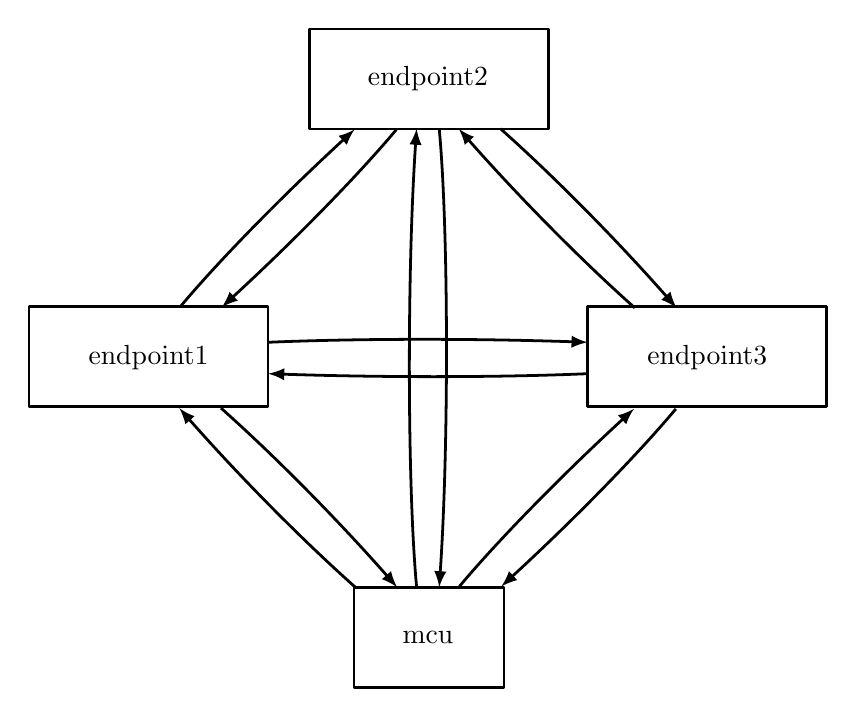
\begin{tikzpicture}[>=latex,line join=bevel,]
  \pgfsetlinewidth{1bp}
%%
\pgfsetcolor{black}
  % Edge: endpoint1 -> mcu
  \draw [->] (70.104bp,101.54bp) .. controls (87.951bp,85.688bp) and (111.04bp,62.583bp)  .. (133.5bp,37.045bp);
  % Edge: endpoint3 -> endpoint2
  \draw [->] (219.07bp,137.63bp) .. controls (201.22bp,153.48bp) and (178.13bp,176.59bp)  .. (155.67bp,202.13bp);
  % Edge: endpoint2 -> endpoint3
  \draw [->] (170.69bp,202.13bp) .. controls (188.54bp,186.27bp) and (211.63bp,163.17bp)  .. (234.09bp,137.63bp);
  % Edge: endpoint2 -> mcu
  \draw [->] (148.67bp,201.96bp) .. controls (151.95bp,166.73bp) and (152.2bp,89.012bp)  .. (148.65bp,37.021bp);
  % Edge: endpoint3 -> endpoint1
  \draw [->] (202.02bp,113.93bp) .. controls (171.39bp,112.61bp) and (130.08bp,112.49bp)  .. (87.085bp,113.93bp);
  % Edge: endpoint3 -> mcu
  \draw [->] (233.83bp,101.24bp) .. controls (220.38bp,85.166bp) and (197.62bp,61.817bp)  .. (170.98bp,37.304bp);
  % Edge: endpoint1 -> endpoint2
  \draw [->] (55.338bp,137.93bp) .. controls (68.788bp,154.01bp) and (91.548bp,177.36bp)  .. (118.19bp,201.87bp);
  % Edge: endpoint1 -> endpoint3
  \draw [->] (87.156bp,125.24bp) .. controls (117.78bp,126.56bp) and (159.1bp,126.69bp)  .. (202.09bp,125.24bp);
  % Edge: mcu -> endpoint1
  \draw [->] (118.48bp,37.044bp) .. controls (100.64bp,52.898bp) and (77.542bp,76.003bp)  .. (55.086bp,101.54bp);
  % Edge: mcu -> endpoint2
  \draw [->] (140.51bp,37.207bp) .. controls (137.23bp,72.441bp) and (136.97bp,150.16bp)  .. (140.52bp,202.15bp);
  % Edge: mcu -> endpoint3
  \draw [->] (155.92bp,37.346bp) .. controls (169.37bp,53.42bp) and (192.13bp,76.769bp)  .. (218.77bp,101.28bp);
  % Edge: endpoint2 -> endpoint1
  \draw [->] (133.25bp,201.83bp) .. controls (119.8bp,185.75bp) and (97.038bp,162.4bp)  .. (70.397bp,137.89bp);
  % Node: endpoint1
\begin{scope}
  \definecolor{strokecol}{rgb}{0.0,0.0,0.0};
  \pgfsetstrokecolor{strokecol}
  \draw (87bp,138bp) -- (1bp,138bp) -- (1bp,102bp) -- (87bp,102bp) -- cycle;
  \draw (44bp,119.59bp) node {endpoint1};
\end{scope}
  % Node: mcu
\begin{scope}
  \definecolor{strokecol}{rgb}{0.0,0.0,0.0};
  \pgfsetstrokecolor{strokecol}
  \draw (172bp,37bp) -- (118bp,37bp) -- (118bp,1bp) -- (172bp,1bp) -- cycle;
  \draw (144.59bp,19bp) node {mcu};
\end{scope}
  % Node: endpoint3
\begin{scope}
  \definecolor{strokecol}{rgb}{0.0,0.0,0.0};
  \pgfsetstrokecolor{strokecol}
  \draw (288bp,138bp) -- (202bp,138bp) -- (202bp,102bp) -- (288bp,102bp) -- cycle;
  \draw (245.17bp,119.59bp) node {endpoint3};
\end{scope}
  % Node: endpoint2
\begin{scope}
  \definecolor{strokecol}{rgb}{0.0,0.0,0.0};
  \pgfsetstrokecolor{strokecol}
  \draw (188bp,238bp) -- (102bp,238bp) -- (102bp,202bp) -- (188bp,202bp) -- cycle;
  \draw (144.59bp,220.17bp) node {endpoint2};
\end{scope}
%
\end{tikzpicture}

